\section{Physical theory}
\subsection{Basics}\label{sec:basics}

 From empirical studies Pareto has been shown that the higher end of a distribution of money follows the distribution trend\cite{paretoslaw}:
 \begin{align}
 	\omega_m\propto m{-1-\alpha}\label{eq:pareto}
 \end{align} 
Here $\alpha\in[1,2]$. This trend will be analytically studied with a system of micro dynamical relations between a group of financial agents, and the resulting money distribution between them. \\


The system consists of $N$ financial agents. They transfer money between them in pairs of $(i,j)$ and they all start with a fixed amount of money $m_0$. The amount of money is arbitrary. So in this project the amount of money is given in amount of "wealth". Here one wealth is $m_0$ and the symbol used is $\$$. A result from this is that $\langle m\rangle=1\$ $\\

At a time step a pair of agents, $(i,j)$, are chosen at random and let them transact money from $j$ to $i$. The pair is chosen at random so for a specific pair $m_i,m_j$ both $(m_i,m_j)$ and $(m_j,m_i)$ are possible. Money is conserved during the transaction which means that the money $\Delta m$ transfered from $j$ to $i$ has to be equal. This means that the total expression for the transaction can be writen as

\begin{align}
	m_i+m_j=m_i'+m_j'\label{eq:pengerbevart}
\end{align}

This transfer is done by a Randomized Number Generator and in this model none of the agents are left with a debt. To remove the debt from the picture, only a percentage of the money is transfered in stead of a fixed amount.

\begin{align}
	m_j'=\epsilon(m_i+m_j)&&\epsilon\in[0,1]\label{epsiloncrit}
\end{align}

And similar for $m_i'$.
\begin{align*}
	m_j'=(1-\epsilon)(m_i+m_j)&&\epsilon\in[0,1]
\end{align*}

Due to the limitations of $\epsilon$ no agent gets debt, but it is likley that one agent is left with zero $m\geq0$. This system now consists of a conserved amount of money with a transfer criteria. It can be shown that this system, given enough time, will relax towards a Gibbs distribution.\cite{proofgibbsdist}

\begin{align}
	\omega_m=\beta e^{-\beta m}
\end{align}

With

\begin{align}
	\beta=\frac{1}{\langle m\rangle}=\qty[\sum_i\frac{m_i}{N}]^{-1}\label{eq:beta}
\end{align}

This model uses $N=500$. The $500$ agents has to do enough transaction to achieve the above outlined distribution. The article suggests that $10^7$ transactions is enough. \cite{patriarca} To find the final equilibrium distribution $\omega_m$ $10^4$ runs were done and $\omega_m$ was taken as the average of all the recorded $\omega_m$. The distribution of agents is exponential, so plotting the logarithm of the trend should yield a straight line.
\begin{align*}
	\ln(\omega_m)=\ln(\beta e^{-\beta m})\\
	\ln(\omega_m)=\ln(\beta)-\beta m %\label{logarithmicline}
\end{align*}


\subsection{Savings}
\label{sec:savings}

To make the model more realistic complexity is added though a savings term. Now every agent will save a fraction of their wealth $\delta$ before the transaction takes place. The addition of this term will change the distribution of agents so it no longer makes a gibbs distribution.

\begin{align}
	m_i'=\lambda m_i+\epsilon(1-\lambda)(m_i+m_j)\label{savingsterm1}
\end{align}

and similar for $m_j'$.
 
 \begin{align}
	 m_j'=\lambda m_j+(1-\epsilon)(1-\lambda)(m_i+m_j) \label{savingsterm2}
 \end{align}
 
 The two terms in the expressions can be simplified by gathering both the savings term and the trading term in a variable $\delta m=(1-\lambda)(\epsilon m_j-(1-\epsilon)m_i)$
 
 \begin{align*}
	 m_i'=\lambda m_i+\delta m
 \end{align*}
 \begin{align*}
	 m_j'=\lambda m_j+\delta m
 \end{align*}

\subsection{Willingness to trade}

The model has up until now only varied how much is saved and not touched on if they want to trade. From observations it is know that the willingness to trade impacts if a trade takes place or not. Further refinement of the model includes two terms to include in the probability of trading. For this the model follows the work of.\cite{goswami} The model now takes into account that there is a probability

\begin{align}
	p_{ij}\propto \abs{m_i-m_j}^{-\alpha}\label{eq:willingness}
\end{align}

for an interaction to take place between two agents with respectively $m_i$ and $m_j$ wealth. The variable $\alpha$ is larger than zero. If $\alpha$ is zero one get the same model as for \ref{savings}. Several runs will be done with varying $\alpha$ to analyze the effect of the probability term on the expression.

\subsubsection{Normalization}
\label{sec:normalization1}
The expression for the willingness to trade \ref{willingness} is not normalized. If one chooses a value less than one the expression will blow up and the probability becomes larger than one.\\

\begin{figure}[H]
\centering
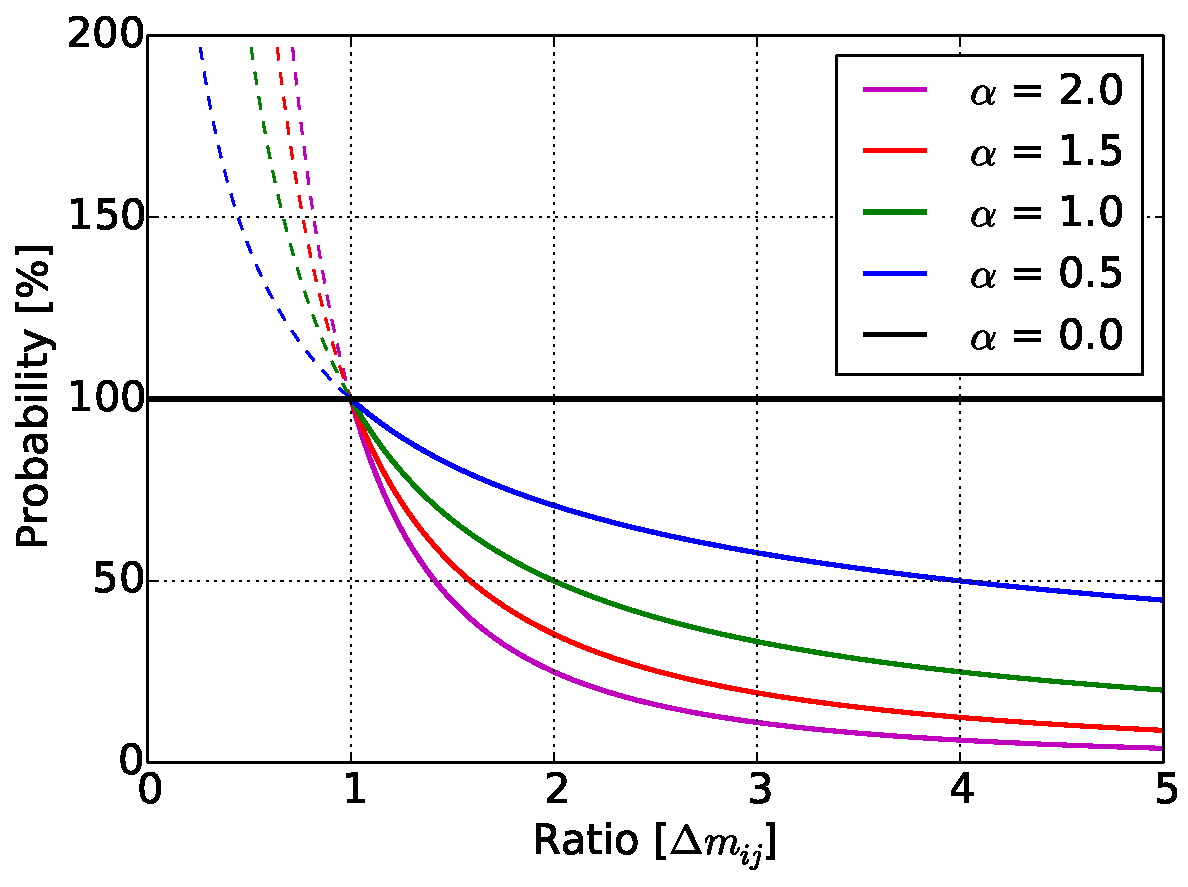
\includegraphics[width=0.7\linewidth]{theory/bilder/difference}
\caption{Figure shows the probability as a function of the difference in wealth between the two agents. The continuous line is the probability chosen in this project while the dashed line shows the trends without the criteria below one.}
\label{fig:difference}
\end{figure}


To prevent unrealistic probabilities above one a normalization criteria is introduced. The suggested normalization criteria on piazza is to normalize it with the expectation value of the agents $\langle m\rangle$.\footnote{\href{https://piazza.com/class/j6owewp05ym46p?cid=126}{\color{blue}{Piazza: Morten's suggestion} }} From \ref{basics} the expectation value $\langle m\rangle=1\$$. So dividing by this will not change this expression. The other change is to add a factor of two to the probability, $2\abs{m_i-m_j}^\alpha/\langle m\rangle$ because the normalization gives an overall decrease in all the probabilities. This is not included because of the way the expectation value is defined here gives no change in the probability. The last piece in the normalization is to remove the probabilities higher than one, although it is not important for this part it will be important in the next section. All probabilities higher than one is synthetically sat to one. The physical representation is that if two agents has a difference in wealth that is less than one, a trade is guarantied.\\

\begin{align} 
p_{ij}=
\left\{\begin{matrix}
|m_i-m_j|^{-\alpha} && |m_i-m_j|>1 \\ 
1 &&|m_i-m_j|<1
\end{matrix}\right.\label{eq:EPICPROB1}
\end{align}

\subsection{Familiarity and trust}
\label{sec:familiarity and trust}
From observations it is known that it is more likely that two agents that know and trust each other trades. In this model this is introduced to the system by adding to the probability a increased probability between agents that has traded earlier.

\begin{align}
	p_{ij}\propto \abs{m_i-m_j}^{-\alpha}\qty(c_{ij}+1)^\gamma\label{eq:roughtrust}
\end{align}

$c_{ij}$ represents the number of previous transactions between the two agents. If $c_{ij}=0$ then the $+1$ factor makes sure that the trust term does not influence the probability. Several runs will be done with varying $\gamma$ to analyze the effect of the modified probability term on the expression.


\subsubsection{Normalization}
\label{sec:normalization2}

As for the term in\ref{sec:normalization1}, the expression above has to be normalized. The normalization criteria suggested in piazza is to divide by the highest amount of trade two agents has traded.\footnote{\href{https://piazza.com/class/j6owewp05ym46p?cid=126}{\color{blue}{Piazza: Morten's suggestion} }}
\begin{align}
p_{ij}= \abs{m_i-m_j}^{-\alpha}\qty(\frac{c_{ij}+1}{c_{\mathrm{max}}+1})^\gamma\label{eq:reformedtrust}
\end{align}
By doing this one would make sure that no value supersedes one.\\

An alternative normalization criteria is to rather than taking the total of all the transactions one could normalize by the average of the two agents maximum value.

\begin{align}
p_{ij}= \abs{m_i-m_j}^{-\alpha}\qty(\frac{c_{ij}+1}{\langle c_{ij \mathrm{, max}}  \rangle + 1})^\gamma\label{eq:BESTtrust}
\end{align}

The physical representation is that when an agent makes a trade it is with respect to what he has previously done, not what what the maximum of all the agents. This will increase the overall probability of a transaction taking place.

\begin{align} 
p_{ij}=
\left\{\begin{matrix}
\abs{m_i-m_j}^{-\alpha}\qty(\frac{c_{ij}+1}{\langle c_{ij \mathrm{, max}}  \rangle + 1})^\gamma\ && |m_i-m_j|>1 \\ 
&&\\
\qty(\frac{c_{ij}+1}{\langle c_{ij \mathrm{, max}}\rangle +1})^\gamma &&|m_i-m_j|<1
\end{matrix}\right.\label{eq:EPICPROB2}
\end{align}

\begin{figure}[H]
\centering
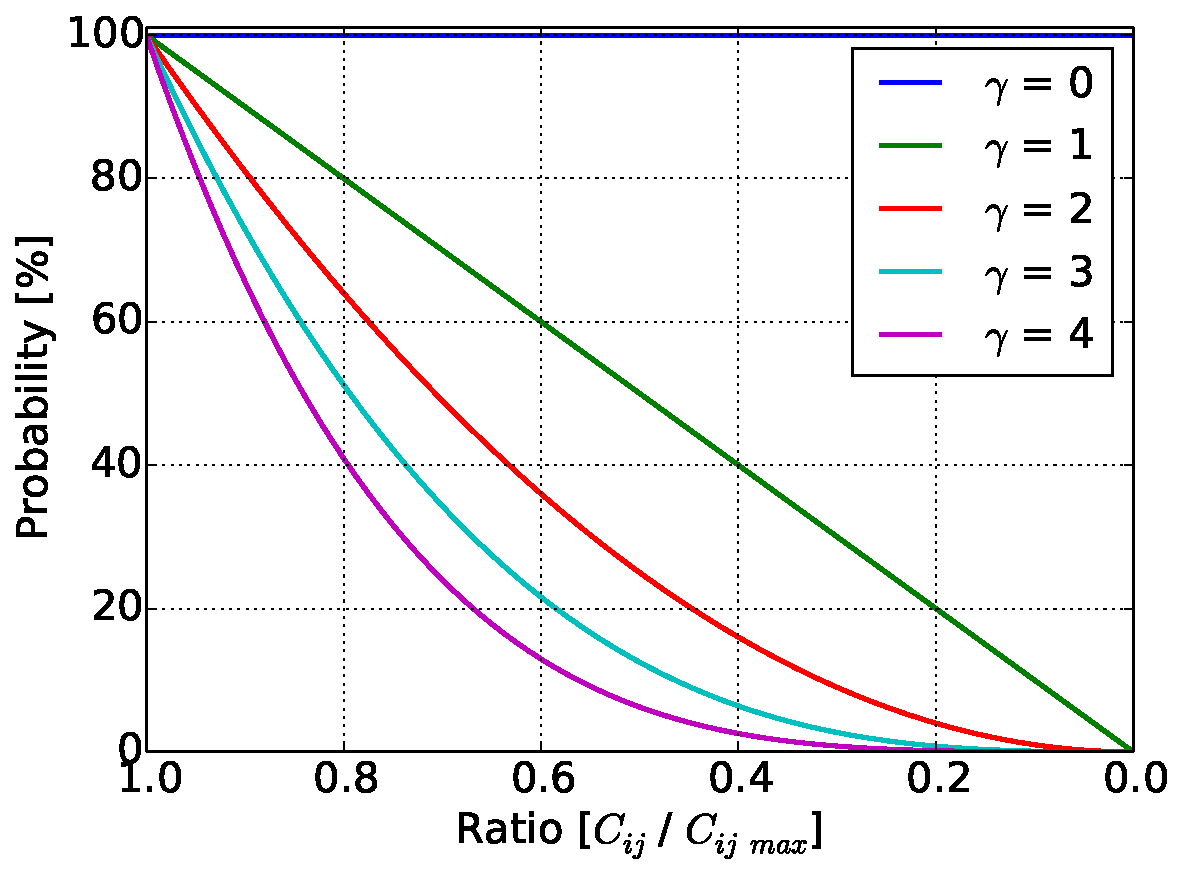
\includegraphics[width=0.5\linewidth]{theory/bilder/interactions}
\caption{Figure shows the probability as a function of their trade ratio.}
\label{fig:interactions}
\end{figure}







